\chapter{固体化学：能带、缺陷与半导体}\label{ch:b3:solid-state}

屋顶上的太阳能板与灯具中的发光二极管，
用的是同一类晶体：硅，或镓与氮、砷、磷的化合物，
并人为掺入每百万个原子中的少量杂质原子。
它们的工作由分子所没有的两样东西决定：能级形成的能带，
带隙的宽度决定晶体吸收或发射哪种光；
另一样是携带电荷的缺陷。
本章由分子轨道构建能带，计算半导体中的载流子数目，
并把缺失的原子与错位的原子当作具有各自平衡的化学物种处理，
直至汽车排气管中氧传感器所用的固体电解质。

\begin{recall}
本科一年级分册定义了晶体、金属键、离子晶体与共价晶体，
间隙位置与合金，以及能斯特方程；本科二年级分册
给出了休克尔方法与共振积分 $\beta$。
在\Cref{ch:b3:x-ray-diffraction}中给出了倒格子，
在\cref{ch:b3:partition-functions}中给出了玻尔兹曼分布和
统计熵 $S = k\ln W$。
\end{recall}

\begin{omfigure}
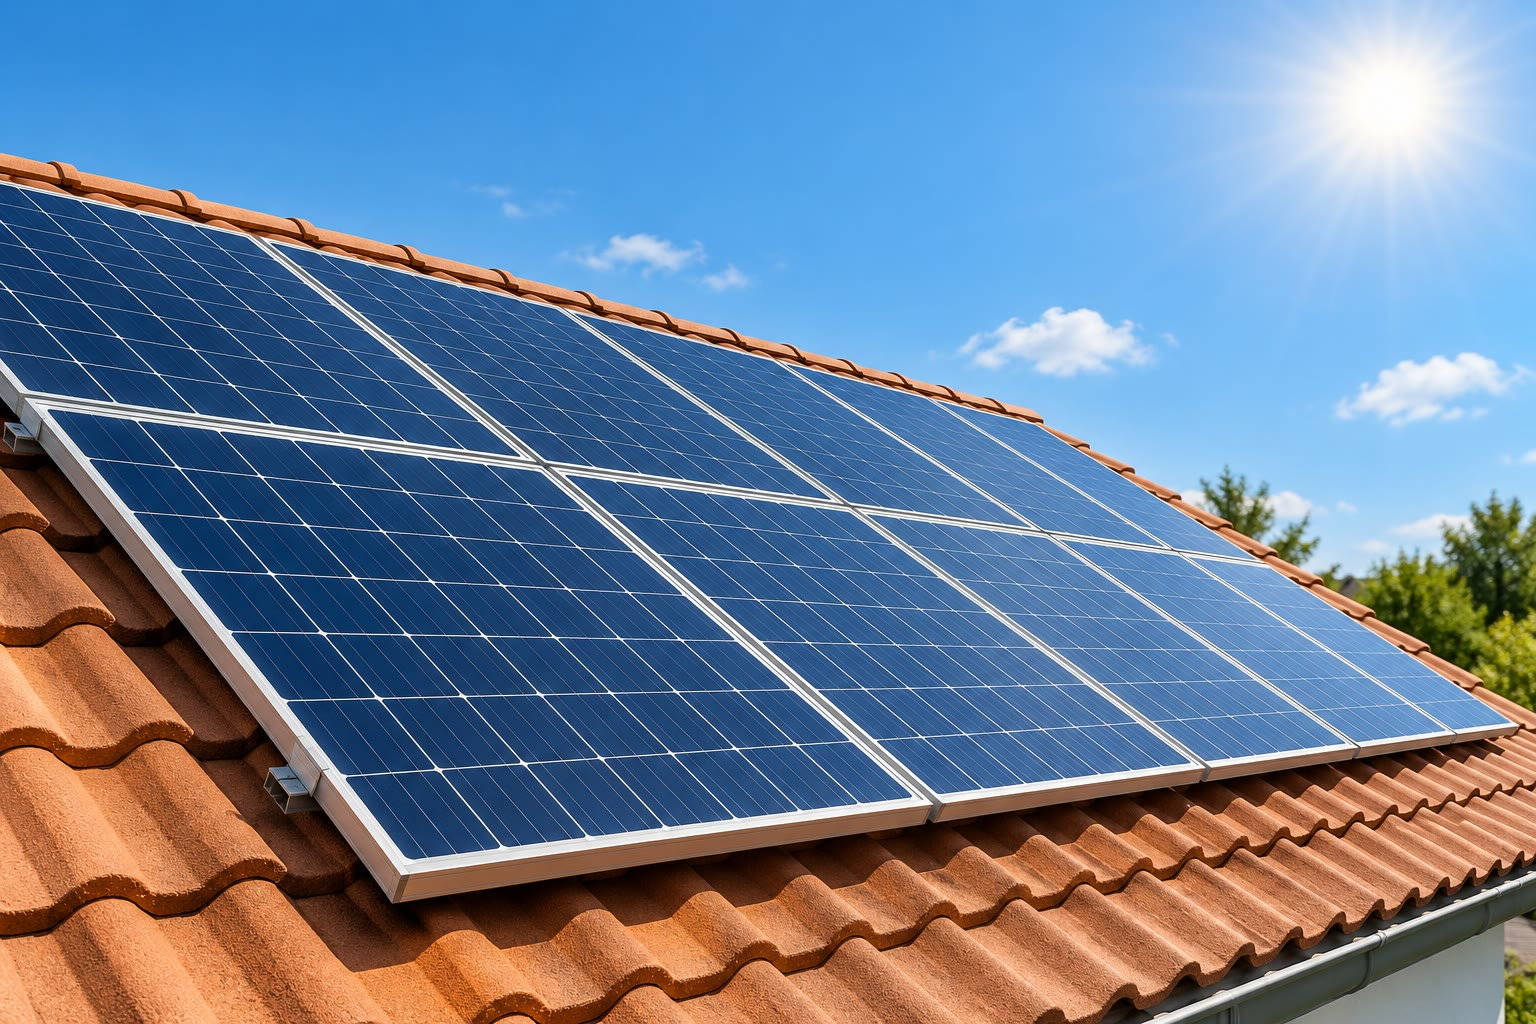
\includegraphics[width=0.6\linewidth]{images/book4/ai/b3-22-solar-panels.jpg}

{\small 瓦屋顶上的太阳能板：每个电池片都是一薄片硅，
光在其中把电子激发越过约一电子伏特的带隙。}
\end{omfigure}

\section{从轨道到能带}

取一条由 $N$ 个相同原子组成的链，每个原子上有一个 s 轨道，在休克尔近似下：
每个原子上的库仑积分为 $\alpha$，
相邻原子间的共振积分为 $\beta < 0$，其余为零。

\begin{theorem}[休克尔链的能级]\label{thm:b3:solid-state:chain}
由 $N$ 个原子构成的线性链有 $N$ 个分子轨道，其能量为
\[
  E_k = \alpha + 2\beta\cos\frac{k\pi}{N + 1}, \qquad k = 1, \dots, N,
\]
系数为 $c_j^{(k)} \propto \sin\bigl(jk\pi/(N + 1)\bigr)$，位于第 $j$ 个原子上。当 $N \to \infty$ 时，能级
在区间 $\alpha + 2\beta$ 到 $\alpha - 2\beta$ 内稠密分布，形成宽度为 $4|\beta|$ 的能带。
\end{theorem}

\begin{proof}
久期方程为 $\beta c_{j-1} + (\alpha - E)c_j + \beta c_{j+1} = 0$，$j = 1, \dots, N$，且 $c_0 = c_{N+1} = 0$
（该处无原子）。取 $c_j = \sin(j\theta)$，由于 $\sin((j - 1)\theta) + \sin((j + 1)\theta) = 2\cos\theta\sin(j\theta)$，
各方程化为 $(\alpha - E + 2\beta\cos\theta)\sin(j\theta) = 0$，故 $E = \alpha + 2\beta\cos\theta$。条件 $c_0 = 0$
对每个 $\theta$ 均成立；$c_{N+1} = \sin((N + 1)\theta) = 0$ 要求 $\theta = k\pi/(N + 1)$；$k = 1, \dots, N$ 给出 $N$ 个互不相同的
能级（其余取值或重复这些能级，或为零）。最低与最高能级为
$\alpha \pm 2\beta\cos(\pi/(N + 1))$，二者趋于 $\alpha \pm 2\beta$；相邻能级的间距至多为
$2|\beta|\pi/(N + 1)$，该值趋于零。
\end{proof}

当 $N = 2$ 时，该定理给出 $\alpha \pm \beta$，即乙烯的 $\pi$ 体系的轨道；
当 $N = 6$ 时，给出开链己三烯。在三维情形中，
同样的情况适用于每一种原子轨道：s 轨道形成 s 能带，p 轨道形成 p 能带，
且每个能带可容纳 $2N$ 个电子（$N$ 为原子数）。

\begin{definition}[能带]\label{def:b3:solid-state:band}
晶体的\emph{能带}\index{能带}是一段连续的
允许单电子能量范围，由晶体中所有原子的轨道形成。
\emph{带隙}\index{带隙} $E_g$ 是两个能带之间
没有能级的能量范围。在零温的半导体或绝缘体中，
最高的已填满能带为\emph{价带}\index{价带}，最低的空能带为
\emph{导带}\index{导带}。
\end{definition}

\begin{definition}[态密度与费米能级]\label{def:b3:solid-state:fermi}
\emph{态密度}\index{态密度} $g(E)$ 是能量 $E$ 附近
单位能量（以及每个原子或单位体积）内的能级数目。
\emph{费米能级}\index{费米能级} $E_F$ 是能级被占据的
概率为 $1/2$ 时所对应的能量；在零温下，低于它的能级全部被填满，
高于它的能级全部为空。
\end{definition}

\begin{omfigure}
\begin{tikzpicture}
\begin{axis}[width=0.78\linewidth, height=6.2cm, xmin=0.3, xmax=7.6, ymin=-2.3, ymax=2.3,
  axis lines=left, xtick={1,2,3,4,5,6.6}, xticklabels={2,4,8,16,64,$\infty$: $g(E)$},
  xlabel={原子数 $N$}, ylabel={$(E - \alpha)/|\beta|$},
  ytick={-2,-1,0,1,2}, tick label style={font=\small}, label style={font=\small}]
\addplot[only marks, mark=-, mark size=7pt, omDef, thick] table[x=col, y=e] {figdata/out/bachelor-3-band-chain.dat};
\addplot[omThm, thick] table[x expr=6.0+0.55*\thisrow{g}, y=e] {figdata/out/bachelor-3-band-chain-b.dat};
\draw[black!40, dashed] (axis cs:0.3,-2) -- (axis cs:7.6,-2);
\draw[black!40, dashed] (axis cs:0.3,2) -- (axis cs:7.6,2);
\draw[<->, black!60] (axis cs:5.6,-2) -- (axis cs:5.6,2) node[midway, left, font=\scriptsize] {$4|\beta|$};
\end{axis}
\end{tikzpicture}

{\small 链长为 2 至 64 个原子的休克尔能级（每条短线表示一个能级；
当 $\beta < 0$ 时，成键能级位于底部）。能级聚成一个能带，
位于 $\alpha + 2\beta$ 与 $\alpha - 2\beta$ 之间；右侧为无限长
链的态密度，在能带边缘处最大。}
\end{omfigure}

\begin{proposition}[能带填充]\label{prop:b3:solid-state:filling}
最高占据能带部分填满的晶体，像金属一样导电；
能带全满或全空、且能带之间存在带隙的晶体，
在零温下不导电。
\end{proposition}

\begin{proof}[论证]
在电场中，电子获得少量能量和动量：它们必须
跃迁到紧邻其占据能级之上的空能级。在部分填满的
能带中，这样的能级紧邻费米能级之上，无需付出能量代价。在全满的
能带中每个能级都已被占据，下一个空能级位于带隙另一侧；
而且，全满的能带不携带净电流，因为每个向一方运动的电子，
都有另一个电子向相反方向运动。
\end{proof}

钠每个原子有一个 3s 电子，其 s 能带半满：是金属。
镁每个原子有两个电子，恰好可以填满其 s 能带，但 s 带与 p 带
相互重叠，因此镁也是金属。金刚石与硅每个原子有四个价电子，
它们所占的轨道分裂为一个全满的成键带和一个空的反键带，
两者之间被带隙隔开。

\begin{definition}[半导体与绝缘体]\label{def:b3:solid-state:classes}
\emph{半导体}\index{半导体}是指带隙足够小（至多约 \qty{3}{eV}）的固体，
在常温下或掺杂后，有可测数量的电子能够跨越该带隙；
\emph{绝缘体}\index{绝缘体}的带隙则很大，
以至于不导电。
\end{definition}

\begin{omfigure}
\begin{tikzpicture}[font=\small]
  \foreach \x/\name in {0/金属, 3.6/半导体, 7.2/绝缘体} {
    \node[font=\small\bfseries] at (\x+0.8,4.3) {\name};
  }
  % metal: one partly filled band
  \fill[omDef!55] (0,0.4) rectangle (1.6,2.0);
  \draw (0,0.4) rectangle (1.6,3.4);
  \draw[omThm, thick] (-0.25,2.0) -- (1.85,2.0) node[right, font=\scriptsize] {$E_F$};
  % semiconductor: small gap
  \fill[omDef!55] (3.6,0.4) rectangle (5.2,1.7);
  \draw (3.6,0.4) rectangle (5.2,1.7);
  \draw (3.6,2.5) rectangle (5.2,3.8);
  \draw[omThm, thick] (3.35,2.1) -- (5.45,2.1) node[right, font=\scriptsize] {$E_F$};
  \draw[<->] (4.4,1.7) -- (4.4,2.5) node[pos=0.8, right, font=\scriptsize] {$E_g$};
  % insulator: large gap
  \fill[omDef!55] (7.2,0.4) rectangle (8.8,1.2);
  \draw (7.2,0.4) rectangle (8.8,1.2);
  \draw (7.2,3.2) rectangle (8.8,4.0);
  \draw[omThm, thick] (6.95,2.2) -- (9.05,2.2) node[right, font=\scriptsize] {$E_F$};
  \draw[<->] (8.0,1.2) -- (8.0,3.2) node[pos=0.75, right, font=\scriptsize] {$E_g$};
  \node[font=\scriptsize, anchor=east] at (3.5,1.05) {价带};
  \node[font=\scriptsize, anchor=east] at (3.5,3.15) {导带};
  \draw[->] (-0.6,0.2) -- (-0.6,3.9) node[above, font=\scriptsize] {$E$};
\end{tikzpicture}

{\small 零温下的能带填充情况（已填充的能级着色）。金属具有部分填充的能带，
其费米能级位于该能带之内；半导体与绝缘体的价带全满、导带全空，
费米能级位于带隙之中，
前者带隙窄，后者带隙宽。}
\end{omfigure}

\section{半导体}

\begin{definition}[载流子]\label{def:b3:solid-state:carriers}
\emph{本征半导体}\index{本征半导体}是指纯净的半导体，
其载流子全部来自跨越带隙被激发的电子。
\emph{载流子}\index{载流子}是能够携带电流的可动粒子，
即导带中的电子，或价带中的\emph{空穴}\index{空穴}，
即价带中的空能级，它如同正电荷一样运动。
\end{definition}

\begin{theorem}[本征载流子浓度]\label{thm:b3:solid-state:intrinsic}
设 $N_c$ 与 $N_v$ 分别为导带与价带的有效态密度，
（在本阶段不加证明地承认），则费米能级距任一能带边缘超过几个 $kT$ 的半导体，
其电子浓度与空穴浓度为
\[
  n = N_c\,\eu^{-(E_c - E_F)/kT}, \qquad p = N_v\,\eu^{-(E_F - E_v)/kT},
\]
而在本征半导体中
\[
  n = p = n_i = \sqrt{N_cN_v}\,\eu^{-E_g/2kT}.
\]
\end{theorem}

\begin{proof}
能量为 $E$ 的能级被占据的概率为 $f(E) = 1/(1 + \eu^{(E - E_F)/kT})$。当
$E - E_F \gg kT$ 时，$f \approx \eu^{-(E - E_F)/kT}$，即玻尔兹曼尾。对导带中的能级求和，
$n = \int g_c(E)\eu^{-(E - E_F)/kT}\,\dd E = \eu^{-(E_c - E_F)/kT}\int g_c(E)\eu^{-(E - E_c)/kT}\,\dd E$，由定义知最后的积分即为
$N_c$。空穴为空能级，在价带中其概率为 $1 - f \approx \eu^{-(E_F - E)/kT}$，
同样的步骤给出 $p$。于是 $np = N_cN_v\eu^{-(E_c - E_v)/kT} = N_cN_v\eu^{-E_g/kT}$，而在纯净晶体中，
每个被激发的电子都留下一个空穴：$n = p$，因此 $n = \sqrt{np}$。
\end{proof}

\begin{proposition}[质量作用定律]\label{prop:b3:solid-state:mass-action}
在任何处于平衡态的半导体中，无论是否掺杂，均有 $np = n_i^2$。
\end{proposition}

\begin{proof}
乘积 $np = N_cN_v\eu^{-E_g/kT}$ 是在
\cref{thm:b3:solid-state:intrinsic}的证明中得到的，它不含 $E_F$：
无论由什么决定费米能级，它都相同，并等于其本征值 $n_i^2$。
它是反应 $\text{无} \rightleftharpoons \mathrm e^- + \mathrm h^+$ 的平衡常数，类似于水的离子积。
\end{proof}

\begin{omfigure}
% ledger: eg:Si.E0, eg:Si.a, eg:Si.b, eg:Ge.E0, eg:Ge.a, eg:Ge.b, dos:Si.Nc, dos:Si.Nv, dos:Ge.Nc, dos:Ge.Nv, dop:Si.P
\begin{tikzpicture}
\begin{axis}[name=a, width=0.45\linewidth, height=5.6cm, xmin=1.2, xmax=4.2, ymin=4, ymax=18,
  axis lines=left, xlabel={$1000\,\mathrm K/T$}, ylabel={$\log_{10}(n_i/\unit{cm^{-3}})$},
  tick label style={font=\scriptsize}, label style={font=\small}]
\addplot[omDef, thick] table[x=invT, y=lgSi] {figdata/out/bachelor-3-semiconductor-carriers.dat};
\addplot[omThm, thick] table[x=invT, y=lgGe] {figdata/out/bachelor-3-semiconductor-carriers.dat};
\node[font=\scriptsize, omDef] at (axis cs:3.4,8.3) {Si};
\node[font=\scriptsize, omThm, anchor=south west] at (axis cs:3.4,14.0) {Ge};
\end{axis}
\begin{axis}[at={(a.east)}, anchor=west, xshift=1.7cm, width=0.45\linewidth, height=5.6cm,
  xmin=1, xmax=25, ymin=10, ymax=17, axis lines=left,
  xlabel={$1000\,\mathrm K/T$}, ylabel={$\log_{10}(n/\unit{cm^{-3}})$},
  tick label style={font=\scriptsize}, label style={font=\small}]
\addplot[omDef, thick] table[x=invT, y=lgn] {figdata/out/bachelor-3-semiconductor-carriers-b.dat};
\addplot[black!45, dashed, unbounded coords=jump, restrict y to domain=10:17] table[x=invT, y=lgni] {figdata/out/bachelor-3-semiconductor-carriers-b.dat};
\node[font=\scriptsize, anchor=west] at (axis cs:2.6,16.4) {本征};
\node[font=\scriptsize] at (axis cs:12,15.35) {饱和，$n = N_D$};
\node[font=\scriptsize] at (axis cs:20,13.2) {冻析};
\end{axis}
\end{tikzpicture}

{\small 左图：硅和锗的本征载流子浓度随
$1/T$ 的变化（模型采用实测能隙和有效态密度）；
斜率接近 $-E_g/2k$。右图为掺入
$\qty{1e15}{cm^{-3}}$ 磷的硅中电子：低温时施主能级保留其电子
（冻析），约 150 至 \qty{500}{K} 时全部电离（$n = N_D$），
高温时本征载流子（虚线，$n_i$）起主导作用。}
\end{omfigure}

\begin{definition}[直接带隙与间接带隙]\label{def:b3:solid-state:gap-types}
若半导体价带顶与导带底位于相同的电子动量处，则称其具有
\emph{直接带隙}\index{直接带隙}，此时仅靠光子即可使电子
越过带隙；若二者动量不同，则称其具有
\emph{间接带隙}\index{间接带隙}，此时跃迁还需
借助晶格振动。
\end{definition}

% ledger: eg:Si, eg:Ge, eg:GaAs, eg:GaN, eg:GaP
硅（\qty{1.12}{eV}）与锗（\qty{0.66}{eV}）具有间接带隙：
它们在较厚的一层中能较好地吸收光，因而适合用作太阳能电池，但
发光能力很差。砷化镓（\qty{1.42}{eV}）与氮化镓（约
\qty{3.4}{eV}）具有直接带隙，是红外与蓝光发光二极管及激光器的基础；
磷化镓（\qty{2.26}{eV}）为间接带隙，但掺杂后可发绿光。
许多颜料的颜色也取决于带隙：
晶体吸收所有满足 $h\nu > E_g$ 的光子，因此带隙位于蓝色区域的硫化镉
呈黄色。

\begin{definition}[掺杂]\label{def:b3:solid-state:doping}
称\emph{掺杂剂}\index{掺杂剂}为人为掺入半导体中的外来原子，
其用量很少，用以提供载流子。在\emph{n 型
半导体}\index{n 型半导体}中，掺杂剂比被替代的原子多一个价电子（如硅中掺磷），
该电子经紧靠导带下方的
\emph{施主能级}\index{施主能级}交给导带；
在\emph{p 型半导体}\index{p 型半导体}中，掺杂剂比被替代的原子少一个价电子
（如硅中掺硼），从价带中接受一个电子进入
紧贴价带上方的\emph{受主能级}\index{受主能级}，留下一个空穴。
\end{definition}

\begin{omfigure}
\begin{tikzpicture}[font=\small]
  \foreach \x in {0, 5.2} {
    \fill[omDef!35] (\x,0) rectangle (\x+3.6,1.0);
    \fill[omDef!12] (\x,2.6) rectangle (\x+3.6,3.6);
    \node[font=\scriptsize] at (\x+1.8,0.5) {价带};
    \node[font=\scriptsize] at (\x+1.8,3.1) {导带};
  }
  \foreach \i in {0,...,5} { \draw[omThm, thick] (0.25+\i*0.55,2.35) -- (0.6+\i*0.55,2.35); }
  \node[font=\scriptsize, anchor=west] at (0.1,1.95) {施主能级，低于导带 \qty{0.045}{eV}};
  \draw[->, omThm] (0.42,2.42) -- (0.42,2.9);
  \fill[omThm] (0.42,2.95) circle (1.6pt);
  \foreach \i in {0,...,5} { \draw[omMeth, thick] (5.45+\i*0.55,1.25) -- (5.8+\i*0.55,1.25); }
  \node[font=\scriptsize, anchor=west] at (5.3,1.6) {受主能级，高于价带 \qty{0.045}{eV}};
  \draw[->, omMeth] (5.62,0.7) -- (5.62,1.18);
  \draw[omMeth, fill=white] (5.62,0.62) circle (1.8pt);
  \node[font=\small\bfseries] at (1.8,4.0) {n 型：Si 中掺 P};
  \node[font=\small\bfseries] at (7.0,4.0) {p 型：Si 中掺 B};
\end{tikzpicture}

{\small 硅能隙中的施主能级与受主能级（能隙未按比例绘制：
掺杂能级距能带边缘约 0.045 eV，能隙为 1.12 eV）。
施主将其电子（圆点）交给导带；受主从价带中
夺取一个电子，留下空穴（圆圈）。}
\end{omfigure}

% ledger: dop:Si.P, dop:Si.B
磷的施主能级位于硅导带下方 \qty{0.045}{eV} 处，
室温下该值小于 $2kT$，硼的受主能级高出价带的能量与之相近，
即在 \qty{300}{K} 时几乎所有掺杂原子均已电离。这正说明
为何每 $10^7$ 个硅原子中仅掺入一个掺杂原子（$\qty{5e15}{cm^{-3}}$），
便能使电子浓度提高几十万倍。

\begin{method}[掺杂半导体的载流子]\label{met:b3:solid-state:doping}
\begin{enumerate}
  \item 检查温度是否处于饱和区（掺杂原子完全
        电离，$N_D \gg n_i$）：则多数载流子为 $n \approx N_D$（或 $p \approx N_A$）。
  \item 由质量作用定律求出少数载流子：$p = n_i^2/N_D$。
  \item 确定费米能级：$E_c - E_F = kT\ln(N_c/n)$，或相对于本征能级，
        $E_F - E_i = kT\ln(n/n_i)$。
  \item 若两种掺杂剂同时存在，则取差值 $N_D - N_A$。
\end{enumerate}
\end{method}

\begin{definition}[pn 结]\label{def:b3:solid-state:junction}
称\emph{pn 结}\index{pn 结}为同一晶体内
p 型区与 n 型区之间的交界面。
\end{definition}

在 pn 结处，电子由 n 侧向 p 侧扩散，空穴则
向相反方向扩散，于是留下一个载流子耗尽的薄层，其中
固定的电离掺杂原子建立起电场；平衡时两侧费米能级
相同。外加电压的一种方向会降低势垒，使电流
通过；反向则提高势垒，此即二极管。在发光二极管中，电子
与空穴注入结区后复合，发出能量
接近 $E_g$ 的光子；在太阳能电池中，结附近吸收的光子产生
电子–空穴对，经电场分离后，电流在
外电路中流动。

\begin{omfigure}
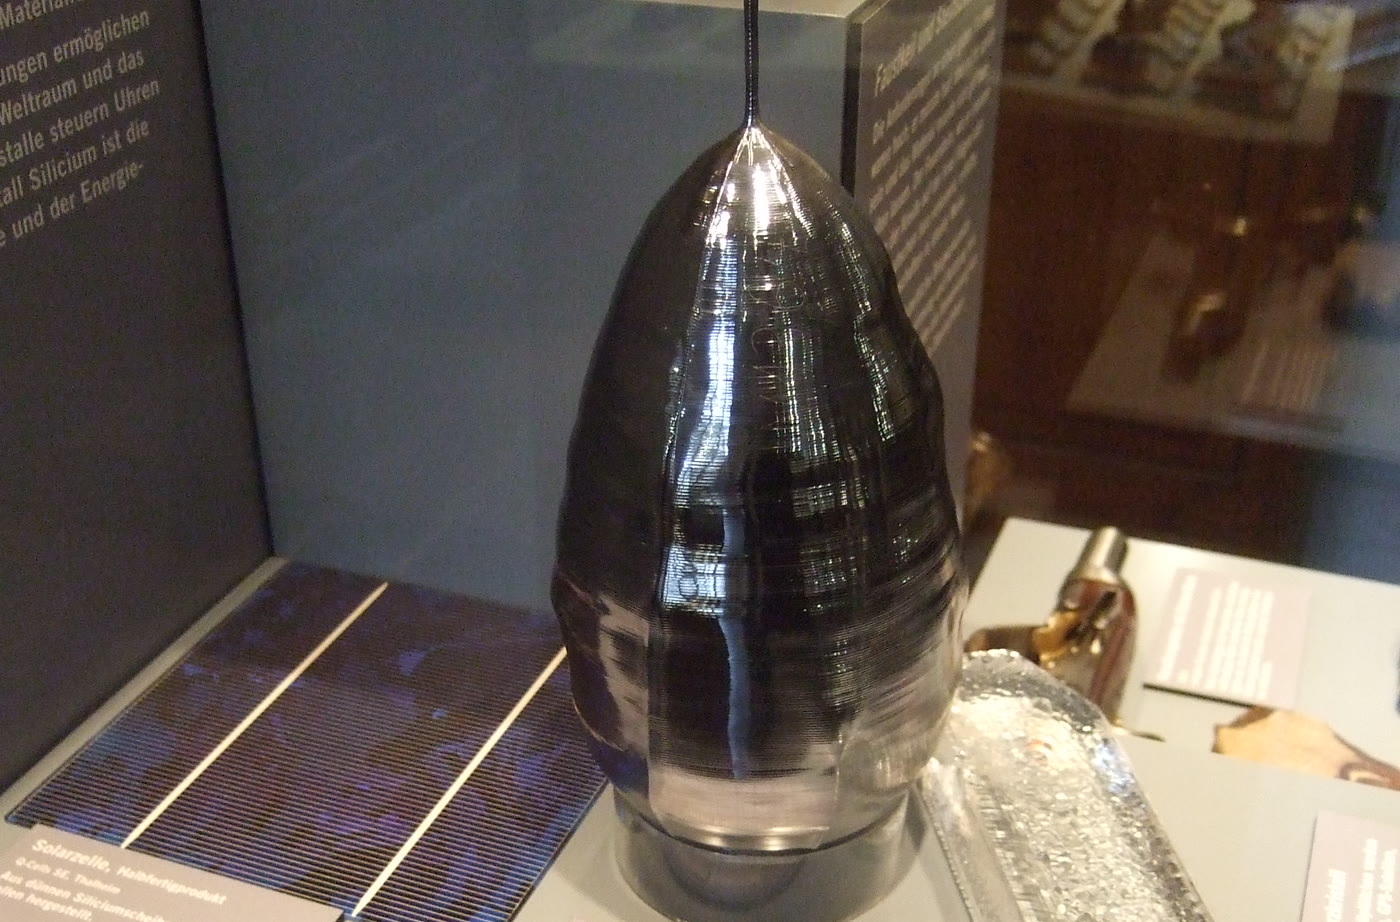
\includegraphics[width=0.5\linewidth]{images/book4/silicon-boule.jpg}

{\small 由熔体中拉制出的单晶硅，旁边展示的是
由该类晶体切片制成的太阳能电池。照片：Sebastian Wallroth，
公有领域。}
\end{omfigure}

\begin{inthelab}[硅单晶的生长]
采用直拉法时，将极纯的多晶硅置于氩气保护的
石英坩埚中熔化，温度略高于熔点，并将掺杂剂
加入熔体中。一根装在旋转杆上的小籽晶浸入
熔体中并缓慢向上提拉：硅沿籽晶的取向在其上结晶，
拉速与转速决定晶体的直径。硅锭
随后被切割成厚度不足一毫米的硅片。硅烷及后续工序所用的掺杂气体
磷化氢和砷化氢均属自燃物质或剧毒物质，
只能在密闭的工业装置中操作。
\end{inthelab}

\section{点缺陷}

\begin{definition}[点缺陷]\label{def:b3:solid-state:defects}
局限于某一格点处、偏离理想晶体的缺陷称为\emph{点缺陷}\index{点缺陷}，
包括空位、间隙原子和杂质原子。在离子晶体中，
\emph{肖特基缺陷}\index{肖特基缺陷}是一对空位，
即一个阳离子空位与一个阴离子空位，其离子已迁移到表面；
\emph{弗仑克尔缺陷}\index{弗仑克尔缺陷}是由一个空位及留下该空位的离子构成的一对缺陷，
该离子位于间隙位置上。
\end{definition}

\begin{omfigure}
\begin{tikzpicture}[scale=0.62]
  \begin{scope}
  \foreach \i in {0,...,5} \foreach \j in {0,...,4} {
    \pgfmathtruncatemacro{\pty}{mod(\i+\j,2)}
    \ifnum\pty=0 \fill[omDef!70] (\i,\j) circle (0.2); \else \fill[omThm!25] (\i,\j) circle (0.38); \draw[omThm!60] (\i,\j) circle (0.38); \fi
  }
  \fill[white] (2,2) circle (0.45); \draw[dashed] (2,2) circle (0.3);
  \fill[white] (3,2) circle (0.45); \draw[dashed] (3,2) circle (0.38);
  \node[font=\small\bfseries] at (2.5,5.0) {肖特基（NaCl）};
  \end{scope}
  \begin{scope}[xshift=8cm]
  \foreach \i in {0,...,5} \foreach \j in {0,...,4} {
    \pgfmathtruncatemacro{\pty}{mod(\i+\j,2)}
    \ifnum\pty=0 \fill[black!45] (\i,\j) circle (0.2); \else \fill[omMeth!25] (\i,\j) circle (0.38); \draw[omMeth!60] (\i,\j) circle (0.38); \fi
  }
  \fill[white] (2,2) circle (0.3); \draw[dashed] (2,2) circle (0.22);
  \fill[black!45] (2.5,2.5) circle (0.2);
  \draw[->, thick] (2.1,2.1) -- (2.38,2.38);
  \node[font=\small\bfseries] at (2.5,5.0) {弗仑克尔（AgCl）};
  \end{scope}
\end{tikzpicture}

{\small 岩盐型晶体某一层中的点缺陷（小点：阳离子；大圆：阴离子；虚线：空位）。
左：肖特基缺陷对，缺失一个阳离子和一个阴离子。右：弗仑克尔缺陷对，
一个银离子从其格点移至
间隙位置。}
\end{omfigure}

\begin{theorem}[肖特基缺陷的平衡浓度]\label{thm:b3:solid-state:schottky}
设晶体 MX 含 $N$ 个化学式单元，平衡时肖特基缺陷对的数目 $n$，
每对的生成焓为 $\Delta H_S$，且 $n \ll N$，则
\[
  \frac{n}{N} = \eu^{-\Delta H_S/2kT}.
\]
\end{theorem}

\begin{proof}
产生 $n$ 对缺陷需耗能 $n\,\Delta H_S$，并由此产生构型熵，
其中阳离子空位的选取方式有 $\binom{N}{n}$ 种，阴离子空位同样多，
故 $S = 2k\ln\frac{N!}{n!(N - n)!}$。利用斯特林公式 $\ln x! \approx x\ln x - x$，
\[
  G(n) = n\,\Delta H_S - 2kT\bigl[N\ln N - n\ln n - (N - n)\ln(N - n)\bigr].
\]
平衡时 $\dd G/\dd n = 0$，即 $\Delta H_S - 2kT\ln\frac{N - n}{n} = 0$，于是 $n/(N - n) = \eu^{-\Delta H_S/2kT}$，因而 $n/N$ 在
$n \ll N$ 时的值。此处忽略缺陷的振动熵，
它只使结果乘以一个常数因子。
\end{proof}

\begin{proposition}[弗仑克尔缺陷]\label{prop:b3:solid-state:frenkel}
设可移动的离子共 $N$ 个，其可占据的间隙位置共 $N_i$ 个，$\Delta H_F$ 为一对缺陷的生成焓，
则弗仑克尔缺陷对的数目为 $n =
\sqrt{NN_i}\,\eu^{-\Delta H_F/2kT}$（$n \ll N, N_i$）。
\end{proposition}

\begin{proof}
此时熵为 $S = k\ln\binom{N}{n} + k\ln\binom{N_i}{n}$，同样的极小化过程给出
\[
  \Delta H_F = kT\ln\frac{(N - n)(N_i - n)}{n^2} \approx kT\ln\frac{NN_i}{n^2},
\]
由此得证。
\end{proof}

平方根表明缺陷成对出现，与半导体中的 $n_i$ 类似，
其浓度的指数中含生成能的一半。碱金属卤化物主要形成
肖特基缺陷；银的卤化物中，小而易极化的
$\ce{Ag+}$ 嵌于阴离子之间，主要形成弗仑克尔缺陷。

\begin{definition}[克罗格–明克符号]\label{def:b3:solid-state:kroger-vink}
\emph{克罗格–明克符号}\index{克罗格–明克符号}将点缺陷写作
$\mathrm{A_S^c}$：A 为格点上的物种（空位记为 V，
间隙位置记为 $i$），S 为它在理想晶体中占据的位置，c 为其相对该位置的电荷：
每个正单位记为 $\bullet$，每个负单位记为 $'$，
无电荷记为 $\times$。
\end{definition}

因此，$\mathrm{V_{Na}'}$ 为钠空位（缺失的 $+1$ 使其相对电荷为 $-1$），
$\mathrm{V_{Cl}^{\bullet}}$ 为氯空位，$\mathrm{Ag_i^{\bullet}}$ 为间隙银离子，$\mathrm{Ca_{Na}^{\bullet}}$ 为占据钠位的钙离子，
$\mathrm{O_O^{\times}}$ 为正常位置上的氧离子。NaCl 的肖特基平衡为
$\text{无} \rightleftharpoons \mathrm{V_{Na}' + V_{Cl}^{\bullet}}$，AgCl 的弗仑克尔平衡为
$\mathrm{Ag_{Ag}^{\times}} \rightleftharpoons \mathrm{Ag_i^{\bullet} + V_{Ag}'}$。

\begin{method}[书写缺陷方程]\label{met:b3:solid-state:kroger-vink}
\begin{enumerate}
  \item 写出加入基质中的物质及其产生的缺陷。
  \item 格点平衡：基质中阳离子格点与阴离子格点之比保持不变
        （空位也计为格点）。
  \item 质量平衡：等式两边原子种类与数目相同（空位无质量；
        电子 $e'$ 与空穴 $h^\bullet$ 同样无质量）。
  \item 电荷平衡：有效电荷之和相等。
\end{enumerate}
\end{method}

\begin{example}[氧化钇在氧化锆中]
将 $\ce{Y2O3}$ 溶入 $\ce{ZrO2}$ 中，使两个 $\ce{Y^3+}$ 占据 $\ce{Zr^4+}$ 位置，每个的相对电荷为 $-1$，并使三个氧离子占据氧位置；
基质中阳离子与氧位置之比为 1:2，
两个阳离子需要四个氧位置，因此其中一个保持空缺：
\[
  \ce{Y2O3} \xrightarrow{\ce{ZrO2}} \mathrm{2\,Y_{Zr}' + 3\,O_O^{\times} + V_O^{\bullet\bullet}}.
\]
格点：2 个阳离子，4 个氧；质量：2 个 Y 与 3 个 O；电荷：$2(-1) + 2 = 0$。
每两个钇离子对应一个氧空位，这正是
使氧化钇稳定氧化锆成为氧离子导体的原因。
\end{example}

\begin{definition}[色心]\label{def:b3:solid-state:colour-centre}
\emph{色心}\index{色心}是一种能吸收
可见光的点缺陷，例如碱金属卤化物中
俘获于阴离子空位的电子（称为 F 中心），它使原本透明的晶体着色。
\end{definition}

将氯化钠在钠蒸气中加热或对其辐照，可产生 F 中心：
被俘获的电子表现得如同尺寸与空位相当的箱中粒子，
吸收可见光，使晶体呈现黄褐色。

\section{非化学计量性}

\begin{definition}[非化学计量化合物]\label{def:b3:solid-state:non-stoichiometric}
\emph{非化学计量化合物}\index{非化学计量化合物}是一种
固体，其组成在一个简单整数比附近的某个范围内变化，
其差额由点缺陷来补偿。
\end{definition}

氧化亚铁从来不是严格的 $\ce{FeO}$：它总是缺铁，
即 $\mathrm{Fe_{1-x}O}$，其中 $x$ 由制备时的温度和氧气压强决定。每缺失一个 $\ce{Fe^2+}$，
就由两个 $\ce{Fe^3+}$ 来补偿，在缺陷语言中，它们即铁格位上的空穴。

\begin{proposition}[电导率与氧气压强]\label{prop:b3:solid-state:brouwer}
对于缺金属氧化物 $\mathrm{M_{1-x}O}$，其缺陷为双电荷金属空位，
由空穴补偿，则空穴浓度及电导率随
$p(\ce{O2})^{1/6}$ 变化。对于缺氧氧化物，由电子补偿，则它们随
$p(\ce{O2})^{-1/6}$ 变化。
\end{proposition}

\begin{proof}
吸收氧气会产生金属空位：
\[
  \tfrac12\ce{O2} \rightleftharpoons \mathrm{O_O^{\times} + V_M'' + 2\,h^{\bullet}}, \qquad K = \frac{[\mathrm{V_M''}][\mathrm h^\bullet]^2}{p(\ce{O2})^{1/2}}
\]
（$\mathrm{O_O^{\times}}$ 的活度为 1）。
电荷平衡为 $[\mathrm h^\bullet] = 2[\mathrm{V_M''}]$，故 $[\mathrm h^\bullet]^3 = 2K\,p(\ce{O2})^{1/2}$，从而 $[\mathrm h^\bullet] \propto p(\ce{O2})^{1/6}$。对于
缺氧情形，$\mathrm{O_O^{\times}} \rightleftharpoons \tfrac12\ce{O2} + \mathrm{V_O^{\bullet\bullet} + 2\,e'}$，$[\mathrm e'] = 2[\mathrm{V_O^{\bullet\bullet}}]$，同样的步骤得 $[\mathrm e'] \propto p(\ce{O2})^{-1/6}$。
电导率与载流子浓度成正比。
\end{proof}

因此，$\log\sigma$ 对 $\log p(\ce{O2})$ 的作图可以指明何种缺陷占主导：其斜率
为 $\pm 1/4$ 或 $\pm 1/6$，取决于缺陷的电荷。

\section{离子导体}

\begin{definition}[离子导体]\label{def:b3:solid-state:ionic-conductor}
\emph{离子导体}\index{离子导体}是一种固体，其中电流
由离子在晶格中迁移来传导。\emph{固体
电解质}\index{固体电解质}是一种离子导体，其电子
电导可以忽略，因而能够将电化学电池的
两个电极隔开。
\end{definition}

\begin{proposition}[离子导电的阿伦尼乌斯定律]\label{prop:b3:solid-state:ionic-arrhenius}
对于在相邻位置之间跃迁、需越过势垒 $E_a$ 的离子，
$\sigma T = A\,\eu^{-E_a/kT}$。
\end{proposition}

\begin{proof}[部分证明]
离子以频率 $\nu_0$ 尝试跳跃，并以概率 $\eu^{-E_a/kT}$ 成功，
因此其扩散系数为 $D = \tfrac16\nu_0 z a^2\eu^{-E_a/kT}$，其中 $z$ 为距离为
$a$ 的相邻位置数（随机游走）。能斯特–爱因斯坦关系 $\sigma = nq^2D/kT$（在本阶段不加证明地承认），
对于单位体积内 $n$ 个电荷为 $q$ 的可动离子，由此得 $\sigma T = (nq^2\nu_0za^2/6k)\,\eu^{-E_a/kT}$。
浓度 $n$ 由掺杂决定（在非本征导体中）；当其
本身由热激发产生时，$E_a$ 中还包含形成焓的一半。
\end{proof}

% ledger: trans:AgI
三种固体电解质展示了这一范围。在氧化钇稳定氧化锆中，
掺杂产生的氧空位使 $\ce{O^2-}$ 离子得以跃迁；它只有在
数百摄氏度的高温下才有实用的导电能力。在 $\beta$-氧化铝中，钠离子
在尖晶石块之间疏松堆积的平面内移动，这是钠–硫
电池的基础。碘化银在高于 \qty{146}{\celsius} 时成为超离子导体，
此时其银离子分布于远多于离子数目的位置上，
几乎如同置于刚性碘化物晶格中的液体。锂离子导体
（锂镧锆石榴石、硫化物）是
目前正在研发的全固态电池的电解质。

\begin{omfigure}
\begin{tikzpicture}[font=\small, >=Stealth]
  \fill[omProp!25] (0,0) rectangle (2.4,3.2);
  \node[font=\scriptsize, align=center] at (1.2,0.6) {$\ce{ZrO2}$--$\ce{Y2O3}$\\ 固体电解质};
  \draw[black!60, line width=2.5pt] (-0.07,0) -- (-0.07,3.2);
  \draw[black!60, line width=2.5pt] (2.47,0) -- (2.47,3.2);
  \node[font=\scriptsize, align=center] at (-2.0,1.4) {废气 \\ $p(\ce{O2})$ 低};
  \node[font=\scriptsize, align=center] at (4.4,1.4) {参比空气 \\ $p(\ce{O2}) = \qty{0.21}{bar}$};
  \node[font=\scriptsize, anchor=north] at (-0.07,-0.05) {Pt};
  \node[font=\scriptsize, anchor=north] at (2.47,-0.05) {Pt};
  \draw[->, thick, omThm] (2.0,1.9) -- (0.4,1.9) node[midway, above, font=\scriptsize] {$\ce{O^2-}$};
  \node[font=\scriptsize, anchor=west] at (2.65,2.75) {$\ce{O2 + 4e- -> 2O^2-}$};
  \node[font=\scriptsize, anchor=east] at (-0.25,2.75) {$\ce{2O^2- -> O2 + 4e-}$};
  \draw (-0.07,3.2) -- (-0.07,4.0) -- (0.85,4.0);
  \draw (2.47,3.2) -- (2.47,4.0) -- (1.55,4.0);
  \draw (1.2,4.0) circle (0.35) node {V};
\end{tikzpicture}

{\small 氧化锆氧传感器的剖面示意：多孔铂电极分置于
固体电解质两面，一个处于废气中，一个处于空气中。
氧离子携带电流通过电解质；电压
测量的是两侧氧气压强之比。}
\end{omfigure}

\begin{history}[晶体管与提拉晶体]
1947 年，约翰·巴丁与沃尔特·布喇顿在威廉·肖克利领导的
贝尔实验室小组中，用一块锗晶体制成了第一只晶体管；三人
共同获得了 1956 年诺贝尔物理学奖。所用晶体来自扬
·切克拉尔斯基于 1916 年发现的方法，他在研究金属结晶速度时，
从熔体中拉出一根锡丝：该方法经改进后用于锗，继而用于硅，
至今仍用于制造几乎所有集成电路的晶片。
\end{history}

\section{练习}

\begin{exercise}[$\star$]\label{exo:b3:solid-state:1}
求由六个原子组成的链的六个休克尔能级（以 $|\beta|$ 为单位），以及
它们所跨越范围的宽度。
\end{exercise}

\begin{exercise}[$\star$]\label{exo:b3:solid-state:2}
由 $N$ 个原子的 s 轨道构成的能带可容纳多少个电子？为什么
钠和镁都是金属？
\end{exercise}

\begin{exercise}[$\star$]\label{exo:b3:solid-state:3}
估算磷化镓发光二极管所发出光的波长，
所用材料分别为磷化镓（\qty{2.26}{eV}）和氮化镓（\qty{3.4}{eV}），利用 $\lambda \approx hc/E_g$ 计算。
\end{exercise}

\begin{exercise}[$\star$]\label{exo:b3:solid-state:4}
写出 $\ce{CaCl2}$ 溶入 $\ce{NaCl}$ 以及 $\ce{Y2O3}$ 溶入 $\ce{ZrO2}$ 的克罗格–明克方程，并
检验每个方程是否配平。
\end{exercise}

\begin{exercise}[$\star\star$]\label{exo:b3:solid-state:5}
已知硅在 \qty{300}{K} 时 $N_c = \num{6.2e15}\,T^{3/2}$，$N_v = \num{3.5e15}\,T^{3/2}$（单位为 $\unit{cm^{-3}}$），$E_g = \qty{1.125}{eV}$；
锗的 $N_c = \num{1.98e15}\,T^{3/2}$，$N_v = \num{9.6e14}\,T^{3/2}$，$E_g = \qty{0.661}{eV}$。分别计算两者的 $n_i$，
并求其比值。
\end{exercise}

\begin{exercise}[$\star\star$]\label{exo:b3:solid-state:6}
硅中掺入 $\qty{1.0e16}{cm^{-3}}$ 的磷。已知
\qty{300}{K} 时 $n_i = \qty{1.0e10}{cm^{-3}}$，求电子和空穴的浓度。
\end{exercise}

\begin{exercise}[$\star\star$]\label{exo:b3:solid-state:7}
对于\cref{exo:b3:solid-state:6}中的晶体，费米能级
比本征能级高多少？
\end{exercise}

\begin{exercise}[$\star\star$]\label{exo:b3:solid-state:8}
NaCl 中一对肖特基缺陷的生成焓约为 \qty{2.3}{eV}（数据见
本练习）。求 \qty{800}{K} 下空位的比例，以及一摩尔中的
缺陷对数。
\end{exercise}

\begin{exercise}[$\star\star$]\label{exo:b3:solid-state:9}
一块氧化亚铁样品（岩盐结构，每个晶胞含四个氧位置）
其 $a = \qty{430.0}{pm}$，密度为 \qty{5.70}{g.cm^{-3}}（数据见本练习）。假设
氧位置全部被占据，求 $x$，化学式写作 $\mathrm{Fe_{1-x}O}$。
\end{exercise}

\begin{exercise}[$\star\star\star$]\label{exo:b3:solid-state:10}
某锂离子导体在 \qty{300}{K} 时 $\sigma = \qty{1.0e-4}{S.cm^{-1}}$，在 \qty{350}{K} 时为 $\qty{7.8e-4}{S.cm^{-1}}$，并
在 \qty{400}{K} 时为 $\qty{3.6e-3}{S.cm^{-1}}$（数据见本练习）。求其活化能。
\end{exercise}

\begin{exercise}[$\star\star\star$]\label{exo:b3:solid-state:11}
证明：在一种氧化物中，主要缺陷为带单位负电荷的金属空位
$\mathrm{V_M'}$，由空穴补偿，电导率正比于 $p(\ce{O2})^{1/4}$。
\end{exercise}

\begin{exercise}[$\star\star\star$]\label{exo:b3:solid-state:12}
在 AgCl 中，弗仑克尔缺陷对的生成焓约为 \qty{1.4}{eV}，每个银离子
对应两个间隙位置（数据见本练习）。计算 \qty{600}{K} 下
处于间隙位置的银离子所占的比例。
\end{exercise}

\section{问题：排气管中的氧传感器}

\begin{problem}[{周末问题——排气管中的氧传感器：钇稳定氧化锆的
缺陷、离子电导率与工作温度，电池的能斯特电压，
以及稀燃与富燃排气之间的切换
}]
\label{pb:b3:solid-state:1}
% ledger: const:R, const:F, const:kB, const:e, const:NA, air:O2
该传感器的电解质为含 8.0\,mol\,\% $\ce{Y2O3}$ 的氧化锆，具有萤石结构，
每个立方晶胞含四个阳离子位置和八个氧位置，$a = \qty{514}{pm}$；一块
厚 \qty{1.0}{mm}、面积为 \qty{0.20}{cm^2} 的圆片将排气与空气隔开。其
电导率满足 $\sigma T = A\eu^{-E_a/kT}$，其中 $E_a = \qty{1.0}{eV}$，在 \qty{800}{\celsius} 时 $\sigma = \qty{0.030}{S.cm^{-1}}$。
稀燃排气中 $p(\ce{O2}) = \qty{0.010}{bar}$，富燃排气中 $p(\ce{O2}) = \qty{1.0e-20}{bar}$（均为本题数据）。

\medskip\noindent\textbf{第一部分——电解质。}
\begin{enumerate}
  \item 写出 $\ce{Y2O3}$ 溶于 $\ce{ZrO2}$ 的克罗格–明克方程。
  \item 检验其位置、质量与电荷的平衡。
  \item 每个钇离子产生多少个氧空位？
  \item 将组成写为 $\mathrm{Zr_{1-x}Y_xO_{2-x/2}}$，并求 $x$。
  \item 计算空置的氧位置所占的比例。
  \item 计算每个晶胞中的空位数。
  \item 计算空位浓度，单位为 $\unit{cm^{-3}}$。
\end{enumerate}

\medskip\noindent\textbf{第二部分——电导率与温度。}
\begin{enumerate}[resume]
  \item 为什么电导率随温度急剧升高？
  \item 求 $A$。
  \item 求 \qty{700}{\celsius} 时的 $\sigma$。
  \item 求 \qty{300}{\celsius} 时的 $\sigma$。
  \item 计算圆片在这两个温度下的电阻。
  \item 电子元件要求电阻低于 \qty{1}{k\ohm}，
        求最低工作温度。
  \item 为什么这类传感器要装配加热器？
\end{enumerate}

\medskip\noindent\textbf{第三部分——能斯特电压。}
\begin{enumerate}[resume]
  \item 写出空气一侧的电极反应，分别用普通表示法和
        克罗格–明克符号表示。
  \item 证明电池电压为 $E = (RT/4F)\ln\bigl(p_{\mathrm{air}}/p_{\mathrm{exh}}\bigr)$。
  \item 计算 \qty{700}{\celsius} 时的 $RT/4F$。
  \item 若排气中含有空气，电压是多少？
  \item 计算 $p(\ce{O2})$ 每变化十倍时电压的变化。
\end{enumerate}

\medskip\noindent\textbf{第四部分——稀燃、富燃与切换。}
\begin{enumerate}[resume]
  \item 计算 \qty{700}{\celsius} 时稀燃排气中的电压。
  \item 计算 \qty{700}{\celsius} 时富燃排气中的电压。
  \item 为什么富燃排气中的 $p(\ce{O2})$ 如此小？
  \item 发动机控制系统在 \qty{0.45}{V} 处切换，这对应
        多大的氧气压强？
  \item 为什么在化学计量空燃比处电压会发生跃变，
        发动机控制如何利用这一点？
  \item 给出结果：\qty{700}{\celsius} 时富燃排气中的传感器电压。
\end{enumerate}
\end{problem}
